\documentclass[12pt]{article}

\usepackage{float}
\usepackage[caption = false]{subfig}
\usepackage{graphicx}
\usepackage{listings}
\usepackage[hidelinks]{hyperref}
\graphicspath{{data/}}

\usepackage{xcolor}
 
\definecolor{codegreen}{rgb}{0,0.6,0}
\definecolor{codegray}{rgb}{0.5,0.5,0.5}
\definecolor{codepurple}{rgb}{0.58,0,0.82}
\definecolor{backcolour}{rgb}{0.95,0.95,0.92}
 
\lstdefinestyle{mystyle}{
    backgroundcolor=\color{backcolour},   
    commentstyle=\color{codegreen},
    keywordstyle=\color{magenta},
    numberstyle=\tiny\color{codegray},
    stringstyle=\color{codepurple},
    basicstyle=\ttfamily\footnotesize,
    breakatwhitespace=false,         
    breaklines=true,                 
    captionpos=b,                    
    keepspaces=true,                 
    numbers=left,                    
    numbersep=5pt,                  
    showspaces=false,                
    showstringspaces=false,
    showtabs=false,                  
    tabsize=2
}
 
\lstset{style=mystyle}

\textheight 23.2 cm

\textwidth 6.0 in

\hoffset = -0.5 in

\voffset = -2.4 cm

\hyphenation{}

\frenchspacing

\title{
\large Introduction to image processing and computer vision \\
\LARGE \textbf{Plant Segmentation and Labeling} \\
Laboratory Project I
}

\author{Patryk Walczak}

\begin{document}

\maketitle

\tableofcontents

\thispagestyle{empty}

\newpage

\clearpage
\pagenumbering{arabic}

\section{Introduction}

\paragraph{
Main task is about finding the best mask for each plant in the dataset (900 images of plants) using image segmentation, the process of splitting the digital image into several objects (segments). More precisely, separate the plant from the background and optionally make the bounding boxes. Then the second part of the project is about dividing the whole plant on distinct leaves, for the better view make each mask of the leaf in a different colour. All results are saved and compared with the patterns.
}

\begin{center}
\begin{figure}[H]
\centering
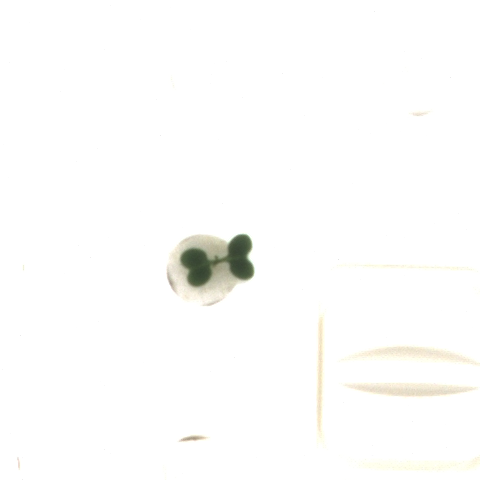
\includegraphics[width = 2.7in]{rgb_00_01_000_00.png}
\hspace{1cm}
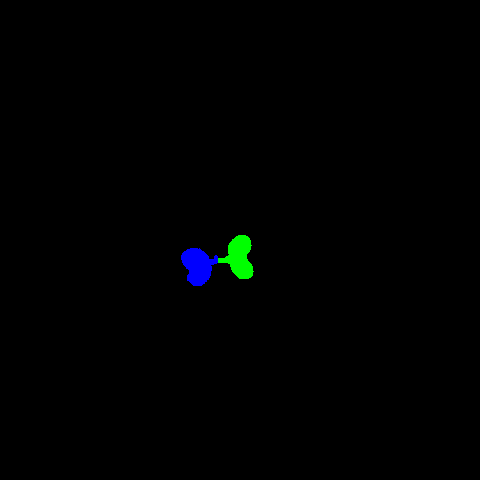
\includegraphics[width = 2.7in]{label_00_01_000_00.png}\\
\vspace{1cm}
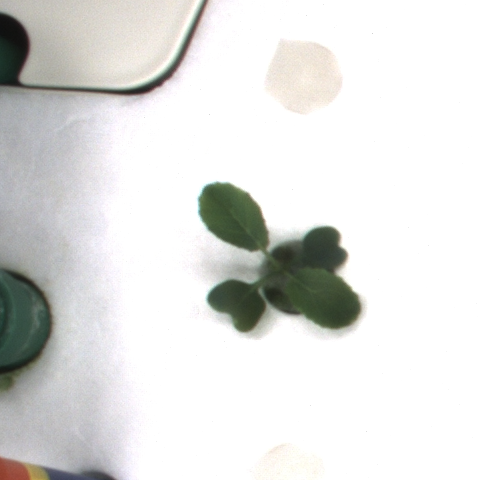
\includegraphics[width = 2.7in]{rgb_00_00_004_01.png}
\hspace{1cm}
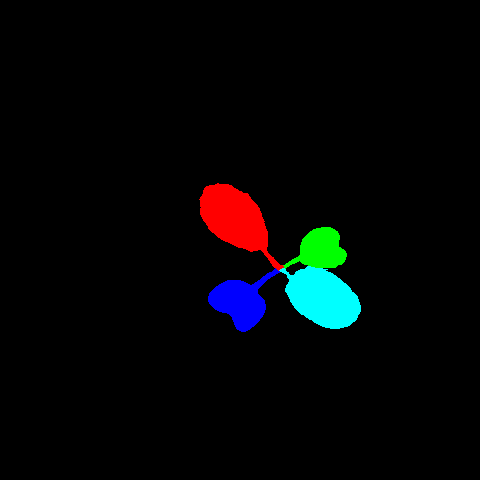
\includegraphics[width = 2.7in]{label_00_00_004_01.png}
\end{figure}
\end{center}

\begin{center}
\begin{figure}[H]
\centering
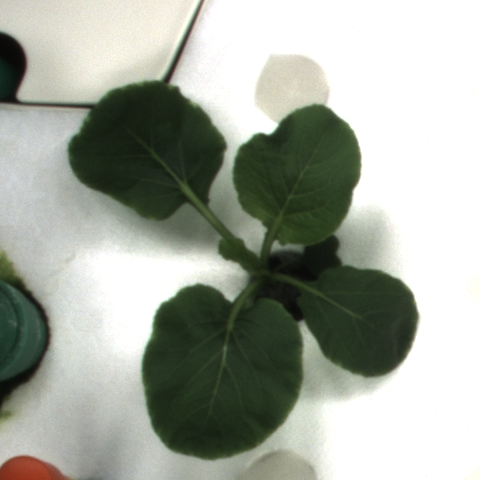
\includegraphics[width = 2.7in]{rgb_01_00_009_05.png}
\hspace{1cm}
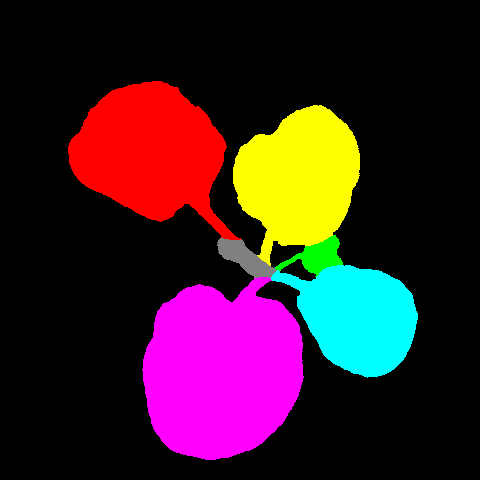
\includegraphics[width = 2.7in]{label_01_00_009_05.png}
\caption{
Some of the images and their patterns
}
\end{figure}
\end{center}


\subsection{Project Description}

\subparagraph{
The dataset contains images of 5 plants made by 3 cameras every 4 hours by 10 days. For the 900 images I prepared several separated files with the algorithms for finding masks, labels, bounding boxes, making comparisons, and for saving the result to the files.\\\\
}

List of files :
\begin{itemize}
\item mask.py - finding the best mask for each image
\item boundingBoxes.py - using the mask to create the bounding box
\item labeling.py - create the separate mask for each leaf
\item saveToFile.py - save masks, labels and bounding boxes to files
\item maskComparison.py - compare my masks with the expectations
\item labelComapison.py - compare my labels with the expectations
\end{itemize}

\newpage

\section{Masks and Bounding Boxes}

\begin{center}
\begin{figure}[h!]
\centering
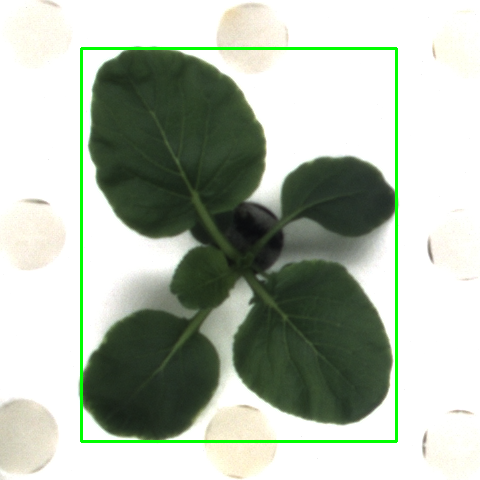
\includegraphics[width = 2in]{box_00_02_009_02.png}
\hspace{1cm}
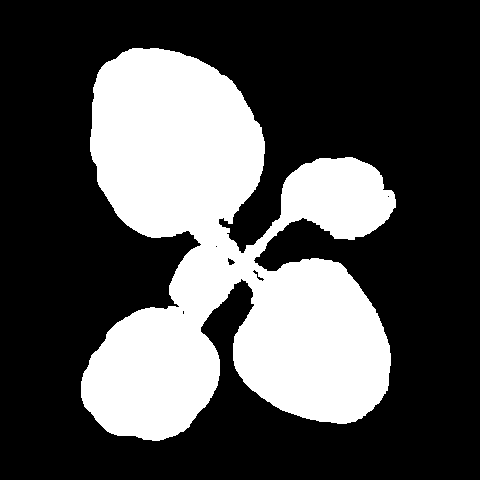
\includegraphics[width = 2in]{rgb_00_02_009_02.png}
\caption{
Example of my results
}
\end{figure}
\end{center}

\subsection{Masks - algorithm description}

Images contain plant on the withe background, which makes the finding mask easier but some of them contain some other green objects also (e.g. bottle), what could be a problem.

\begin{center}
\begin{figure}[h!]
\centering
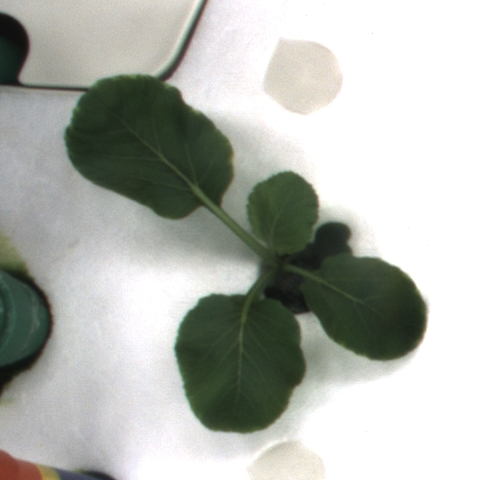
\includegraphics[width = 2in]{rgb_00_00_008_03.png}
\hspace{1cm}
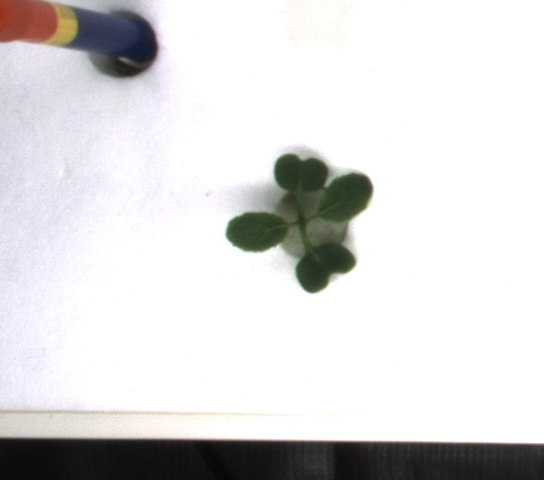
\includegraphics[width = 2in]{rgb_00_04_002_05.png}
\end{figure}
\end{center}

My algorithm as input takes the path to the image and the debug flag.

\begin{lstlisting}[language=Python]
def mask(path, test):
\end{lstlisting}

Firstly my algorithm reads the image with colours, and remove generally all colours except green. For finding the best values for lower and upper array I prepared test.py, where in real-time I could change the values and observe how it affects the mask.\\\\

\newpage

Part of the code. Whole file is in Source Code section.

\begin{lstlisting}[language=Python]
    hsv = cv2.cvtColor(image,cv2.COLOR_BGR2HSV)

    # get info from track bar and apply to result
    hM = cv2.getTrackbarPos('h M','result')
    hL = cv2.getTrackbarPos('h L','result')
    sM = cv2.getTrackbarPos('s M','result')
    sL = cv2.getTrackbarPos('s L','result')
    vM = cv2.getTrackbarPos('v M','result')
    vL = cv2.getTrackbarPos('v L','result')
    # b1 = cv2.getTrackbarPos('blur1','result')
    # b2 = cv2.getTrackbarPos('blur2','result')

    # Normal masking algorithm
    lower = np.array([hL,sL,vL])
    upper = np.array([hM,sM,vM])

    res = cv2.inRange(hsv,lower, upper)
\end{lstlisting}

\begin{lstlisting}[language=Python]
hsv = cv2.cvtColor(image , cv2.COLOR_BGR2HSV)
lower_green = np.array([0, 0, 0],np.uint8)
upper_green = np.array([179, 255, 165],np.uint8)
mask = cv2.inRange(hsv, lower_green , upper_green)
\end{lstlisting}

Only the plant should be taken into consideration, so my algorithm takes the most centre contour. But if the contour is too big it means that the algorithm takes a plant and some other object. So additional removing of the green shades is needed.

\begin{lstlisting}[language=Python]
# finding contur of the biggest area
ret,thresh = cv2.threshold(mask,127,255,0)
contours, hierarchy = cv2.findContours(thresh,cv2.RETR_TREE,\
cv2.CHAIN_APPROX_SIMPLE)
c = sorted(contours, key = cv2.contourArea, reverse = True)[0]

# if the biggest contour has the area > 40000 then remove more precisely
# all colors exept green
if cv2.contourArea(c) > 40000:
segmented = cv2.bitwise_and(image , image , mask=mask)
hsv = cv2.cvtColor(segmented , cv2.COLOR_BGR2HSV)
lower_green = np.array([27, 29, 0],np.uint8)
upper_green = np.array([179, 255, 165],np.uint8)
mask = cv2.inRange(hsv, lower_green , upper_green)
if test :
cv2.imshow("warunek", mask)
cv2.waitKey()
ret,thresh = cv2.threshold(mask,127,255,0)
contours, hierarchy = cv2.findContours(thresh,cv2.RETR_TREE, cv2.CHAIN_APPROX_SIMPLE)
# set minArea = 5000
minArea = 5000
else :
# set minArea = 1000
minArea = 1000
\end{lstlisting}

The variable $minArea$ is specified for each case and it defines the lower bound of the contour's size.\\
Then take the most centered biggest contour with the area bigger than minArea, and save the mask.

\begin{lstlisting}[language=Python]
# finding the generall shape of plant as the most center contour
# of the area > minArea
closest=1000
for c in contours :
if cv2.contourArea(c)>minArea:
M = cv2.moments(c)
cX = int(M["m10"] / M["m00"])
cY = int(M["m01"] / M["m00"])
dist=abs(width/2-cX)+abs(height/2-cY)
if closest > dist:
closest=dist
cnt=c

# take the generall mask of the plant
mask = cv2.drawContours(np.zeros((height ,width ,3), np.uint8 ), [cnt], 0, (255,255,255), cv2.FILLED)
mask = cv2.cvtColor(mask ,cv2.COLOR_BGR2GRAY)
\end{lstlisting}

After that, the algorithm takes the segmented mask to operate only on the plant part.

\begin{lstlisting}[language=Python]
# take only part of the mask from the image
segmented = cv2.bitwise_and(image , image , mask=mask)
\end{lstlisting}

And it applies more precisely removing of the rest green shades. If the step had been used before choosing the plant contour would have been harder because the plant would have been splited in many parts.

\begin{lstlisting}[language=Python]
# more precisely remove all colors exept green
# only from the segmented part of the image
hsv = cv2.cvtColor(segmented , cv2.COLOR_BGR2HSV)
lower_brown = np.array([37, 31, 28],np.uint8)
upper_brown = np.array([86, 255, 134],np.uint8)
mask_seg = cv2.inRange(hsv, lower_brown , upper_brown)
\end{lstlisting}

At the end it applies erosion and dilatation, the number of iterations depends on the area of the biggest contour.

\begin{lstlisting}[language=Python]
# perform a series of erosions and dilations depends on
# the max contour area
kernel22 = cv2.getStructuringElement(cv2.MORPH_RECT, (1,1))
mask_seg = cv2.morphologyEx(mask_seg, cv2.MORPH_OPEN , kernel22)
ret,thresh = cv2.threshold(mask_seg,127,255,0)
contours, hierarchy = cv2.findContours(thresh,cv2.RETR_TREE, cv2.CHAIN_APPROX_SIMPLE)
# take the biggest contur
maxContour = sorted(contours, key = cv2.contourArea, reverse = True)[0]
# set size of the contur devided by 25000
size = int(cv2.contourArea(maxContour)//25000)
# perform erosion and dilatation with size iteration
mask_seg = cv2.erode(mask_seg, None, iterations = size)
mask_seg = cv2.dilate(mask_seg, None, iterations = size)
\end{lstlisting}

Finally, the algorithm returns the mask.

\begin{lstlisting}[language=Python]
# and return the mask of the plant
return mask_seg
\end{lstlisting}

\subsection{Bounding Boxes - algorithm description}

\begin{center}
\begin{figure}[h!]
\centering
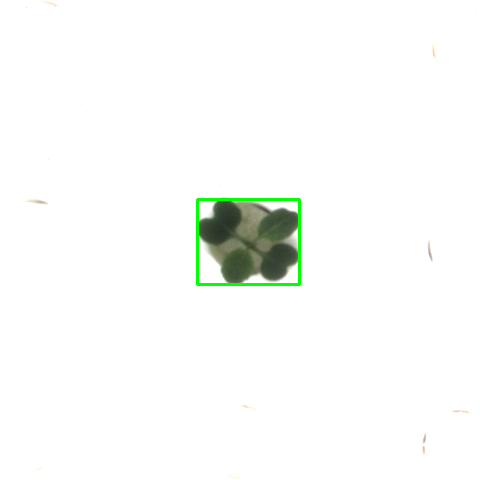
\includegraphics[width = 2in]{box_00_02_002_01.png}
\hspace{1cm}
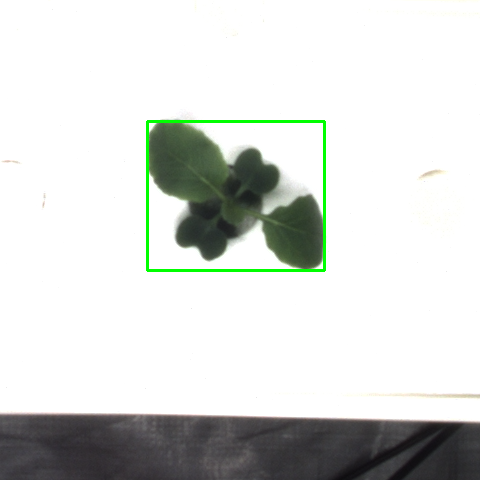
\includegraphics[width = 2in]{box_00_03_005_00.png}
\end{figure}
\end{center}

The algorithm for boxes is very short. It takes the mask and the image, for the mask, prepares the smallest rectangle containing the  whole mask and applies the rectangle to the image.

\begin{lstlisting}[language=Python]
def bounding_boxes(p):
mask = main(p,False)
image = cv2.imread(p,cv2.IMREAD_COLOR)
x,y,w,h = cv2.boundingRect(mask)
cv2.rectangle(image,(x,y),(x+w,y+h),(0,255,0),2)
return image
\end{lstlisting}

\subsection{Saving the results}

\subparagraph{
For saving I prepared separate file, creating directories if those don't exist, and save the result to them. \\\\
}

All result masks are in the directory "my\_mask", and all result bounding boxes are in "my\_bounding\_boxes" directory.

\begin{lstlisting}[language=Python]
directoryMask = 'my_masks'
directoryBoxes = 'my_bounding_boxes'

# save maske
def saveMasks(name):
image = mask(name, False)
name = os.path.basename(name)
cv2.imwrite(pathToWrite+directoryMask+'/'+name, image)

#save label
def saveLabels(name):
image = sum(label(name, False))
name = os.path.basename(name)
cv2.imwrite(pathToWrite+directoryLabel+'/'+name.replace('rgb','label'), image)
\end{lstlisting}


\begin{center}
\begin{figure}[hb!]
\centering
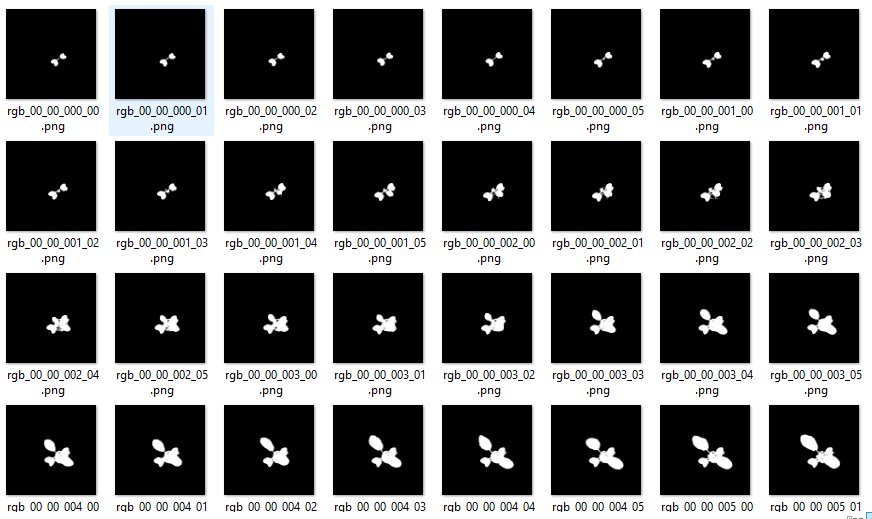
\includegraphics[width = 4in]{directory.png}
\hspace{1cm}
\centering
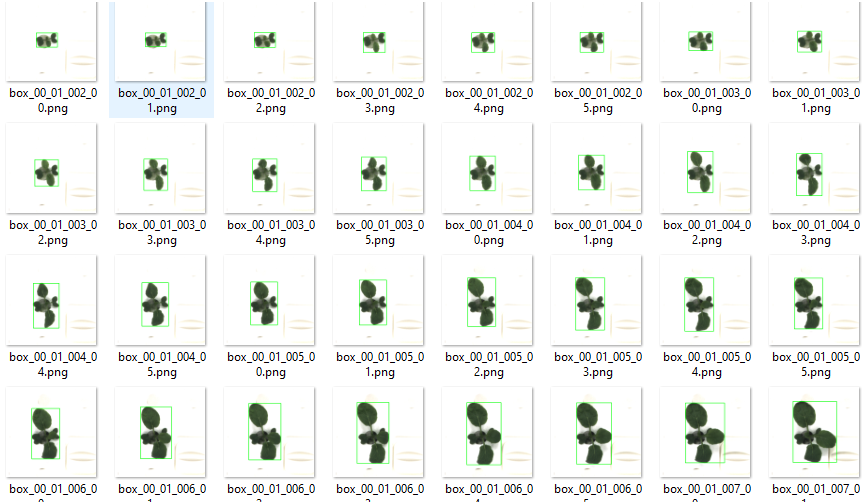
\includegraphics[width = 4in]{directory1.png}
\end{figure}
\end{center}

\subsection{Comparision}

\subparagraph{
I prepared also a new file "maskComparison.py" for checking the final result. Obligatory was including Intersection over Union metric
and Dice coefficient. There are also 2 additional comparisons : Jaccard Index and Structural Similarity Index.\\\\
}

All comparison results are in the directory "ComparisonMasks", in separate files.
Each plant has its result, at the end of each comparison result file there comes its summary. Images are read in the following way:

\newpage

\begin{lstlisting}[language=Python]
# read the pattern
def pattern(path):
image = cv2.imread(pathToPatterns+path)
image = cv2.cvtColor(image, cv2.COLOR_BGR2GRAY)
ret,th1 = cv2.threshold(image,0,255,cv2.THRESH_BINARY)
# return binary mask
return th1

# read my mask
def my_mask(path):
image = cv2.imread(pathToMyMasks+path.replace('label','rgb'))
image = cv2.cvtColor(image, cv2.COLOR_BGR2GRAY)
return image
\end{lstlisting}

And the comparison functions look like:

\begin{lstlisting}[language=Python]
# IoU comparison
def IoU_compare(my_mask,pat):
img1 = np.asarray(pat).astype(np.bool)
img2 = np.asarray(my_mask).astype(np.bool)
num = np.sum(np.logical_and(img1,img2))
den = np.sum(np.logical_or(img1,img2))
return num/den

# dice coefficient coparison
def dice_coeff_compare(my_mask, pat):
img1 = np.asarray(pat).astype(np.bool)
img2 = np.asarray(my_mask).astype(np.bool)
img_intersection = np.bitwise_and(img1, img2)
image_sum = img1.sum() + img2.sum()
if image_sum == 0:
return 0
return 2. * img_intersection.sum() / image_sum

# ssim coparison
def ssim_compare(my_mask, pat):
(score, diff) = compare_ssim(my_mask, pat, full=True)
diff = (diff * 255).astype("uint8")
return score

# jaccard comaprison by function
def jaccard_compare(my_mask, pat):
score = jaccard_similarity_score(my_mask.flatten(), pat.flatten())
return score
\end{lstlisting}

\newpage

Results are also printed at the end of the program.

\begin{center}
\begin{figure}[h!]
\centering
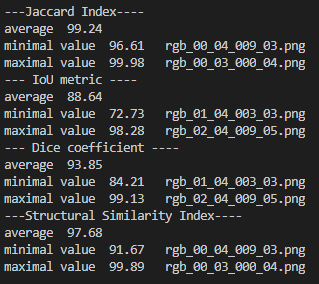
\includegraphics[width = 2.6in]{MaskResult.png}
\hspace{1cm}
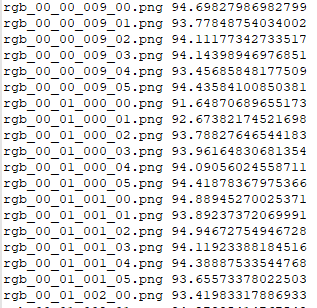
\includegraphics[width = 2.6in]{MaskResult1.png}
\end{figure}
\end{center}

The results are not perfect because in some images the shadow of the plant has the same colour as the part of a leaf. In others,
flowerpot is also green, and it is impossible to remove the pot without erasing the plant. However almost all images are around 90\%, and the worst score is still over 72\%.

\newpage

\section{Segmented Leaves}

\paragraph{
The second part of the project is about segmentating the plant on the leaves.
}

\subsection{Label - algorithm description}

\subparagraph{
The whole described here algorithm is in "labeling.py" file. \\\\
}

Firstly, algorithm takes the result of the previous part, the mask.

\begin{lstlisting}[language=Python]
my_mask = mask(p,False)
\end{lstlisting}

Then it finds the biggest contour and computes the area of the contour.

\begin{lstlisting}[language=Python]
# find the biggest contour
ret,thresh = cv2.threshold(my_mask,127,255,0)
contours, hierarchy = cv2.findContours(thresh,cv2.RETR_TREE,cv2.CHAIN_APPROX_SIMPLE)
maxContour = sorted(contours, key = cv2.contourArea, reverse = True)[0]
maxContourArea = cv2.contourArea(maxContour)
\end{lstlisting}

After that program prepares the variables for next funcitons. The values depends on the area of the max contour.
One of the cases is below.

\begin{lstlisting}[language=Python]
#cases of erosion and dilatalion depends on the area
if maxContourArea < 7500 :
size = int(cv2.contourArea(maxContour)//10000) + 5
erod = size
dilat = 3 * size
minArea = 0
else:
\end{lstlisting}

Then erosion is performed.

\begin{lstlisting}[language=Python]
# pefrome erosion
mask_erode = cv2.erode(my_mask, None, iterations = erod)
\end{lstlisting}

Once again it takes all contours, sorts them and for every one makes the mask, dilatation and segmentation with my\_mask.
Save all of them in list l.

\begin{lstlisting}[language=Python]
contours = sorted(contours, key = cv2.contourArea, reverse=True)
for cnt in contours:
if cv2.contourArea(cnt)>minArea:
# make the mask of the contour and dilate it
m = cv2.drawContours(np.zeros((height ,width ,3), np.uint8 ), [cnt], 0, colors[iter%(len(colors)+1)], cv2.FILLED)
m = cv2.dilate(m, None, iterations = dilat)
# segmented with my_mask
m = cv2.bitwise_and(m, m, mask=my_mask)
iter=iter+1
# add to list
l.append(m)
\end{lstlisting}

\newpage

At the end algorithm removes intersections of the smaller and the bigger mask from the bigger one.

\begin{lstlisting}[language=Python]
# for every mask in list
for i in range(0,len(l)-1):
#from bigger mask remove the intersection with the smaller
l[i] = removeBitwiseMask(l[i], l[i+1])
\end{lstlisting}

Finally, it returns the list of the masks.

\begin{lstlisting}[language=Python]
#return the list of mask
return l
\end{lstlisting}


\subsection{Saving the results}

\subparagraph{
Saving labels is in the same file "saveToFile.py" as in the case of masks. Before saving, the function has to sum all elements of the list returned by $label$ function to save them as one file - as in the patterns.\\\\
}

The saving function is as follows:

\begin{lstlisting}[language=Python]
#save label
def saveLabels(name):
image = sum(label(name, False))
name = os.path.basename(name)
cv2.imwrite(pathToWrite+directoryLabel+'/'+name.replace('rgb','label'), image)
\end{lstlisting}

\begin{center}
\begin{figure}[H]
\centering
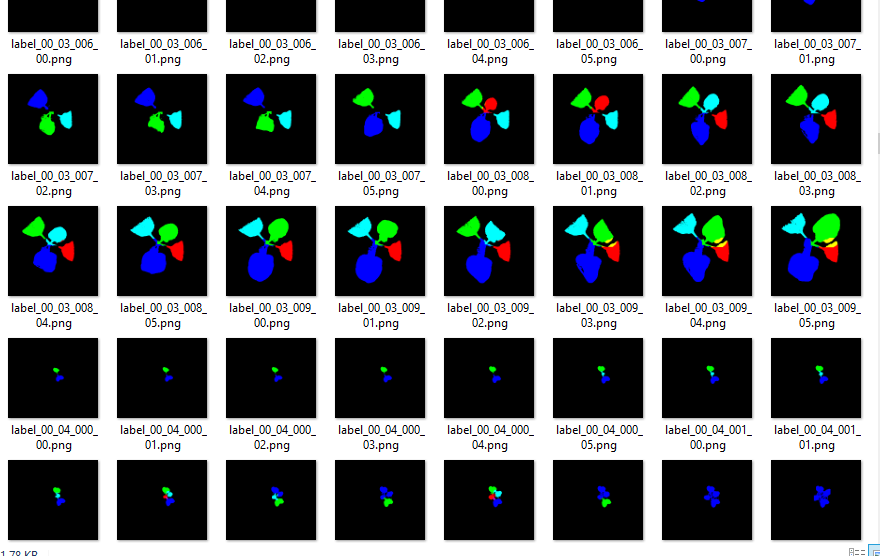
\includegraphics[width = 4in]{directory3.png}
\end{figure}
\end{center}

\newpage

\subsection{Comparision}

\subparagraph{
For comparison labels, I prepared "labelComapison.py". But in the case only the two required comparisons are useful - Intersection over Union metric and Dice coefficient. The two remaining tests are out of point and return score above 90\%, what is false result \\
}

All comparison results are in the directory "ComparisionLabels", in separate files.
Single one consists the data for each for each leaf, for each plant and mean for the whole dataset. But in label case, the comparison is divided on every colour in the pattern.
Each colour mask is separately saved in the dictionary.

\begin{lstlisting}[language=Python]
# read the pattern
def pattern(path):
image = cv2.imread(pathToPatterns+path)
image = cv2.cvtColor(image, cv2.IMREAD_COLOR)
d = dict()
for c in colors:
arr = np.array(c)
res = cv2.inRange(image, arr, arr)
if np.sum(res) > 0:
segmented = cv2.bitwise_and(image , image , mask=res)
d[c] = segmented
return d

# read my mask
def my_label(path, keys):
image = cv2.imread(pathToMyLabels+path)
image = cv2.cvtColor(image, cv2.IMREAD_COLOR)
d = dict()
for c in keys:
arr = np.array(c)
res = cv2.inRange(image, arr, arr)
segmented = cv2.bitwise_and(image , image , mask=res)
d[c] = segmented
return d
\end{lstlisting}

Comparison functions are the same as in mask comparison

\begin{lstlisting}[language=Python]
# IoU comparison
def IoU_compare(my_mask,pat):
img1 = np.asarray(pat).astype(np.bool)
img2 = np.asarray(my_mask).astype(np.bool)
num = np.sum(np.bitwise_and(img1,img2))
den = np.sum(np.bitwise_or(img1,img2))
return num/den

# dice coefficient coparision
def dice_coeff_compare(my_mask, pat):
img1 = np.asarray(pat).astype(np.bool)
img2 = np.asarray(my_mask).astype(np.bool)
img_intersection = np.logical_and(img1, img2)
image_sum = img1.sum() + img2.sum()
if image_sum == 0:
return 0
return 2. * img_intersection.sum() / image_sum
\end{lstlisting}

The result for the whole plant is the mean from the sum of all leaves divided by the number of leaves.

\begin{lstlisting}[language=Python]
for key in pat.keys():
dice[str(name)+str(key)] = dice_coeff_compare(my_l[key], pat[key])
iou[str(name)+str(key)] = IoU_compare(my_l[key], pat[key])
d += dice[str(name)+str(key)]
u += iou[str(name)+str(key)]
file_dice.write(str(name)+" "+str(key)+" "+str(dice[str(name)+str(key)]*100)+"\n")
file_iou.write(str(name)+" "+str(key)+" "+str(iou[str(name)+str(key)]*100)+"\n")
dice[str(name)] = d/len(pat)
iou[str(name)] = u/len(pat)
file_dice.write(str(name)+" "+str(dice[str(name)]*100)+"\n")
file_iou.write(str(name)+" "+str(iou[str(name)]*100)+"\n")
\end{lstlisting}

All results are saved in two files in "ComparisionLabels" directory. At the end of each file are summary containing :  average, minimal and maximal score.

\begin{center}
\begin{figure}[H]
\centering
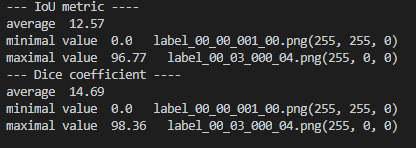
\includegraphics[width = 3in]{LabelsResults.png}

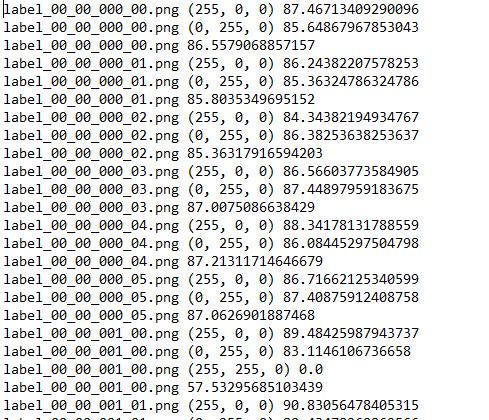
\includegraphics[width = 3in]{LabelsResults1.png}
\end{figure}
\end{center}

The results are far from perfect. The best scores ale close to the results of mask comparison but the average shows that the algorithm  is still not working well.
The reason for that is probably the fact that mask is close to the pattern but the differences are significant. Bad mask of the plant implicates the bad masks for each leaf.\\
Moreover, the choosing of the colour was a big problem. Because the oldest one should have a blue colour. In the algorithm the biggest one is blue. And the comparison firstly divides the images by colours, so a big part of the older plats return in the comparison the result close to 0. The oldest leaf in some photos is under the younger one so its visible area is no longer the biggest. Furthermore, the algorithm considers only one image which implies the problem, with finding the oldest one, hard to solve because nothing on the images marks the age of leaves.
 \\
But taking into consideration only the part with finding the leaves on the image the algorithm does quite well. The result of such a comparison might be close to 40-50\%. This is still not prerfect, but much closer to that.

\section{Source Code}

\subsection{mask.py}
\lstinputlisting[language=Python]{../mask.py}

\subsection{boundingBoxes.py}
\lstinputlisting[language=Python]{../boundingBoxes.py}

\subsection{labeling.py}
\lstinputlisting[language=Python]{../labeling.py}

\subsection{saveToFile.py}
\lstinputlisting[language=Python]{../saveToFile.py}

\subsection{mask.py}
\lstinputlisting[language=Python]{../maskComparison.py}

\subsection{labelComapison.py}
\lstinputlisting[language=Python]{../labelComapison.py}

\subsection{test.py}
\lstinputlisting[language=Python]{../test.py}

\newpage

\section{References}

\begin{enumerate}
\item \url{https://www.overleaf.com/learn/latex/Code\_listing}
\item \url{https://en.wikipedia.org/wiki/Image\_segmentation}
\item \url{https://pythonprogramming.net/color-filter-python-opencv-tutorial/}
\item \url{https://docs.opencv.org/3.4/dd/d49/tutorial\_py\_contour\_features.html}
\item \url{https://docs.opencv.org/2.4/doc/tutorials/imgproc/shapedescriptors/\\bounding\_rects\_circles/bounding\_rects\_circles.html}
\end{enumerate}

\end{document}